\documentclass[]{book}

\usepackage{import}
\usepackage{preamble}
\usepackage{tikz}

\begin{document}

\noindent BECA / Huson / 11.1 IB Math SL \hspace{2in} Name:\\*
20 November 2017
\begin{center}
{\Large Exit Note: Quadratics graphing}\\
\textit{This counts as a participation grade. Answer in the space provided.}
\end{center}

%\vspace{0.2 cm}


\begin{enumerate}

\item Let $f(x) = x^2-2x-3$ and $g(x)=-2x+1$
\begin{enumerate}
    \item Rewrite $f$ in vertex form and state the vertex as an ordered pair.\\*[35pt]
    \item Factor the function $f$ and write down its roots.\\*[35pt]
    \item Graph the function $f$, labeling it. Mark the intercepts and graph the axis of symmetry as a dotted line, labeling it with its equation.
    \item Graph $g$ and label it with its name or equation.
    \item Mark the intersections of $f$ and $g$ as ordered pairs. 

\end{enumerate}


\begin{figure}[!htbp]
\begin{center}
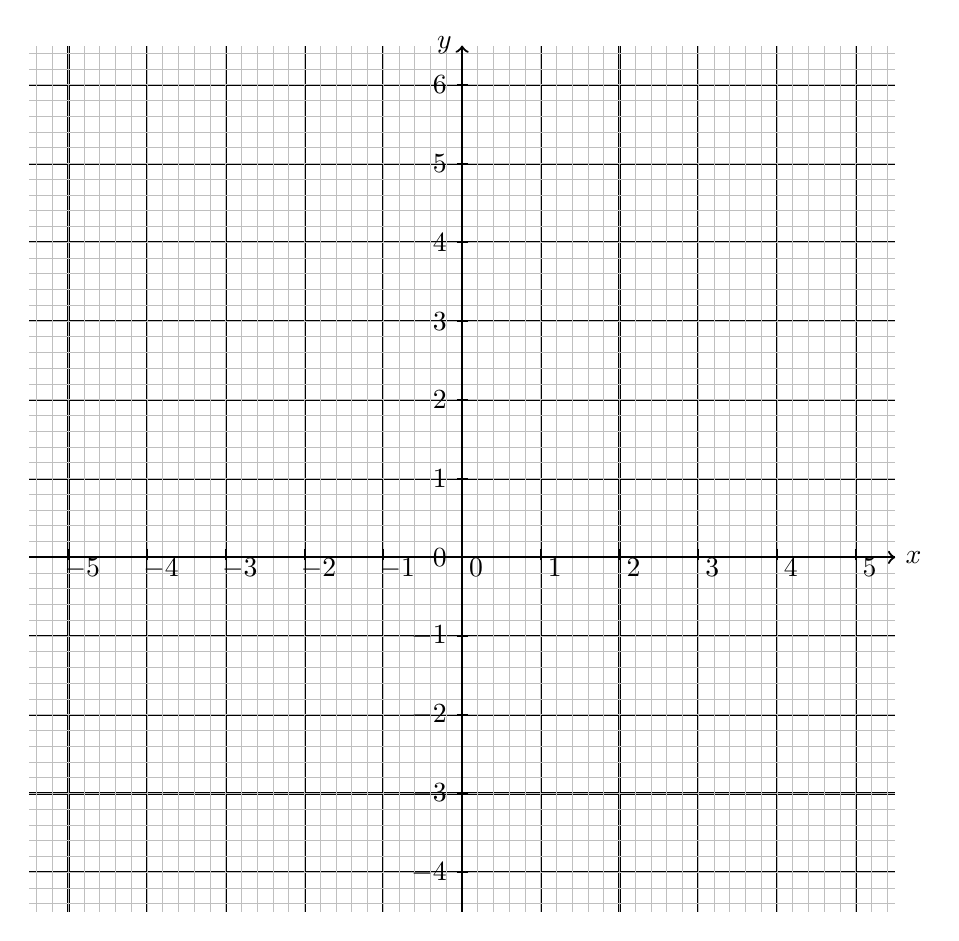
\begin{tikzpicture}

%grid
\draw [thick, color=black,, xstep=1.0cm,ystep=1.0cm] (-5.5,-4.5) grid (5.5,6.5);
\draw [thin, color=lightgray,, xstep=0.2cm,ystep=0.2cm] (-5.5,-4.5) grid (5.5,6.5);

\foreach \x in {-5, -4, -3, -2, -1, 0,1,2,3,4,5}
\draw[shift={(\x,0)},color=black] (0pt,-1pt) -- (0pt,3pt) node[below]  {$\quad \x$};

\foreach \y in {-4, -3, -2,-1,0,1,2,3,4, 5, 6}
\draw[shift={(0,\y)},color=black] (2pt,0pt) -- (-2pt,0pt) node[left]  {$\y$};

\draw [thick, ->] (-5.5,0) -- (+5.5,0) node [right] {$x$};
\draw [thick, ->] (0,-4.5) -- (0,6.5) node [left] {$y$};

%\draw [<-, ->] plot[domain= -5.5:3.5] (\x, 0.5*\x*\x +\x -4);
%\draw [<-, ->] plot[domain= -5.5:3] (\x, -\x-1.5);

\end{tikzpicture}
\end{center}
\end{figure}

\newpage
\noindent BECA / Huson / 11.1 IB Math SL \hspace{2in} Name:\\*
20 November 2017
\begin{center}
{\Large Quiz Corrections: Exponents and radicals}\\
\textit{In addition to correcting your quiz, work these problems. Answer in the space provided.}
\end{center}

%\vspace{0.2 cm}


Simplify, leaving no negative or fractional exponents.



\item $7x^{-2}y \times 3x^3 y^{-1}$\\*[55pt]
\item $\sqrt[5]{a^6 b^{10}}$\\*[55pt]
\item $\displaystyle x^{\frac{1}{2}} \times (\frac{x}{z^6})^{\frac{1}{2}}$\\*[55pt]
\item $\displaystyle (a^6 b^4)^{\frac{1}{3}} \div a^{-3} b^\frac{4}{3}$\\*[55pt]

\newpage
\item Let $f(x) = \sqrt{x} -16$ and $g(x)=(x-4)^4$
\begin{enumerate}
    \item Find $(f \circ g)(x)$\\*[65pt]
    \item Find $f^{-1}(x)$\\*[65pt]
\end{enumerate}

\item The function $f(x)=e^x$ is shown on the graph. Sketch $g(x)=-f(x-4)+3$. Plot and label the asymptotes.

\begin{figure}[!htbp]
\begin{center}
\begin{tikzpicture}

%grid
%\draw [thick, color=black,, xstep=1.0cm,ystep=1.0cm] (-5.5,-1.5) grid (5.5,16.5);
%\draw [thin, color=lightgray,, xstep=0.2cm,ystep=0.2cm] (-5.5,-1.5) grid (5.5,16.5);

\foreach \x in {-5, -4, -3, -2, -1, 0,1,2,3,4,5}
\draw[shift={(\x,0)},color=black] (0pt,-3pt) -- (0pt,3pt) node[below]  {$\x$};

\foreach \y in {-1,0,1,2,3,4,5, 6, 7}
\draw[shift={(0,\y)},color=black] (2pt,0pt) -- (-2pt,0pt) node[left]  {$\y$};

\draw [thick, ->] (-5.5,0) -- (+5.5,0) node [right] {$x$};
\draw [thick, ->] (0,-1.0) -- (0,7.5) node [left] {$y$};

\draw [<-, ->] plot[domain= -3:2] (\x, e^\x);

\end{tikzpicture}
\end{center}
\end{figure}

\end{enumerate}
\end{document}
